\chapter{Конструкторский раздел}
\label{cha:design}

В данном разделе будет проведена конкретизация поставленных задач, составлены и проанализированы алгоритмы.

\section{Функциональная модель}
На рисунке \ref{img:IDEF0} представлена функциональная модель IDEF0 уровня 1.
\begin{figure}
    \centering
    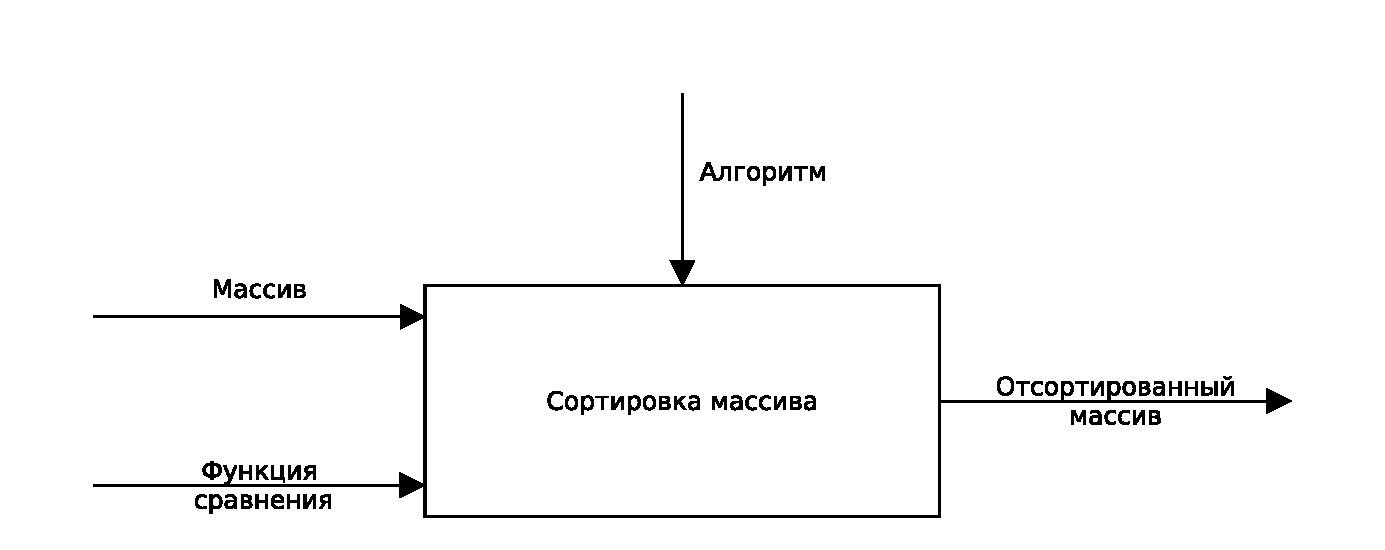
\includegraphics[scale=0.75]{./pdf/mainIdef0.pdf}
    \caption{Функциональная IDEF0 модель уровня 1}
    \label{img:IDEF0}
\end{figure}

\section{Разработка алгоритмов}
Для непосредственной реализации вышеописанных алгоритмов важно иметь их некоторые упрощённые визуальные представления, так как чтение таких представлений упрощает написание кода. Подходящим для этого вариантом визуализации являются схемы алгоритмов.

На рисунках \ref{img:qs}, \ref{img:ins}, \ref{img:shs} изображены схемы алгоритмов быстрой сортировки, сортировки вставками и шейкерной сортировки.

\begin{figure}[H]
    \centering
    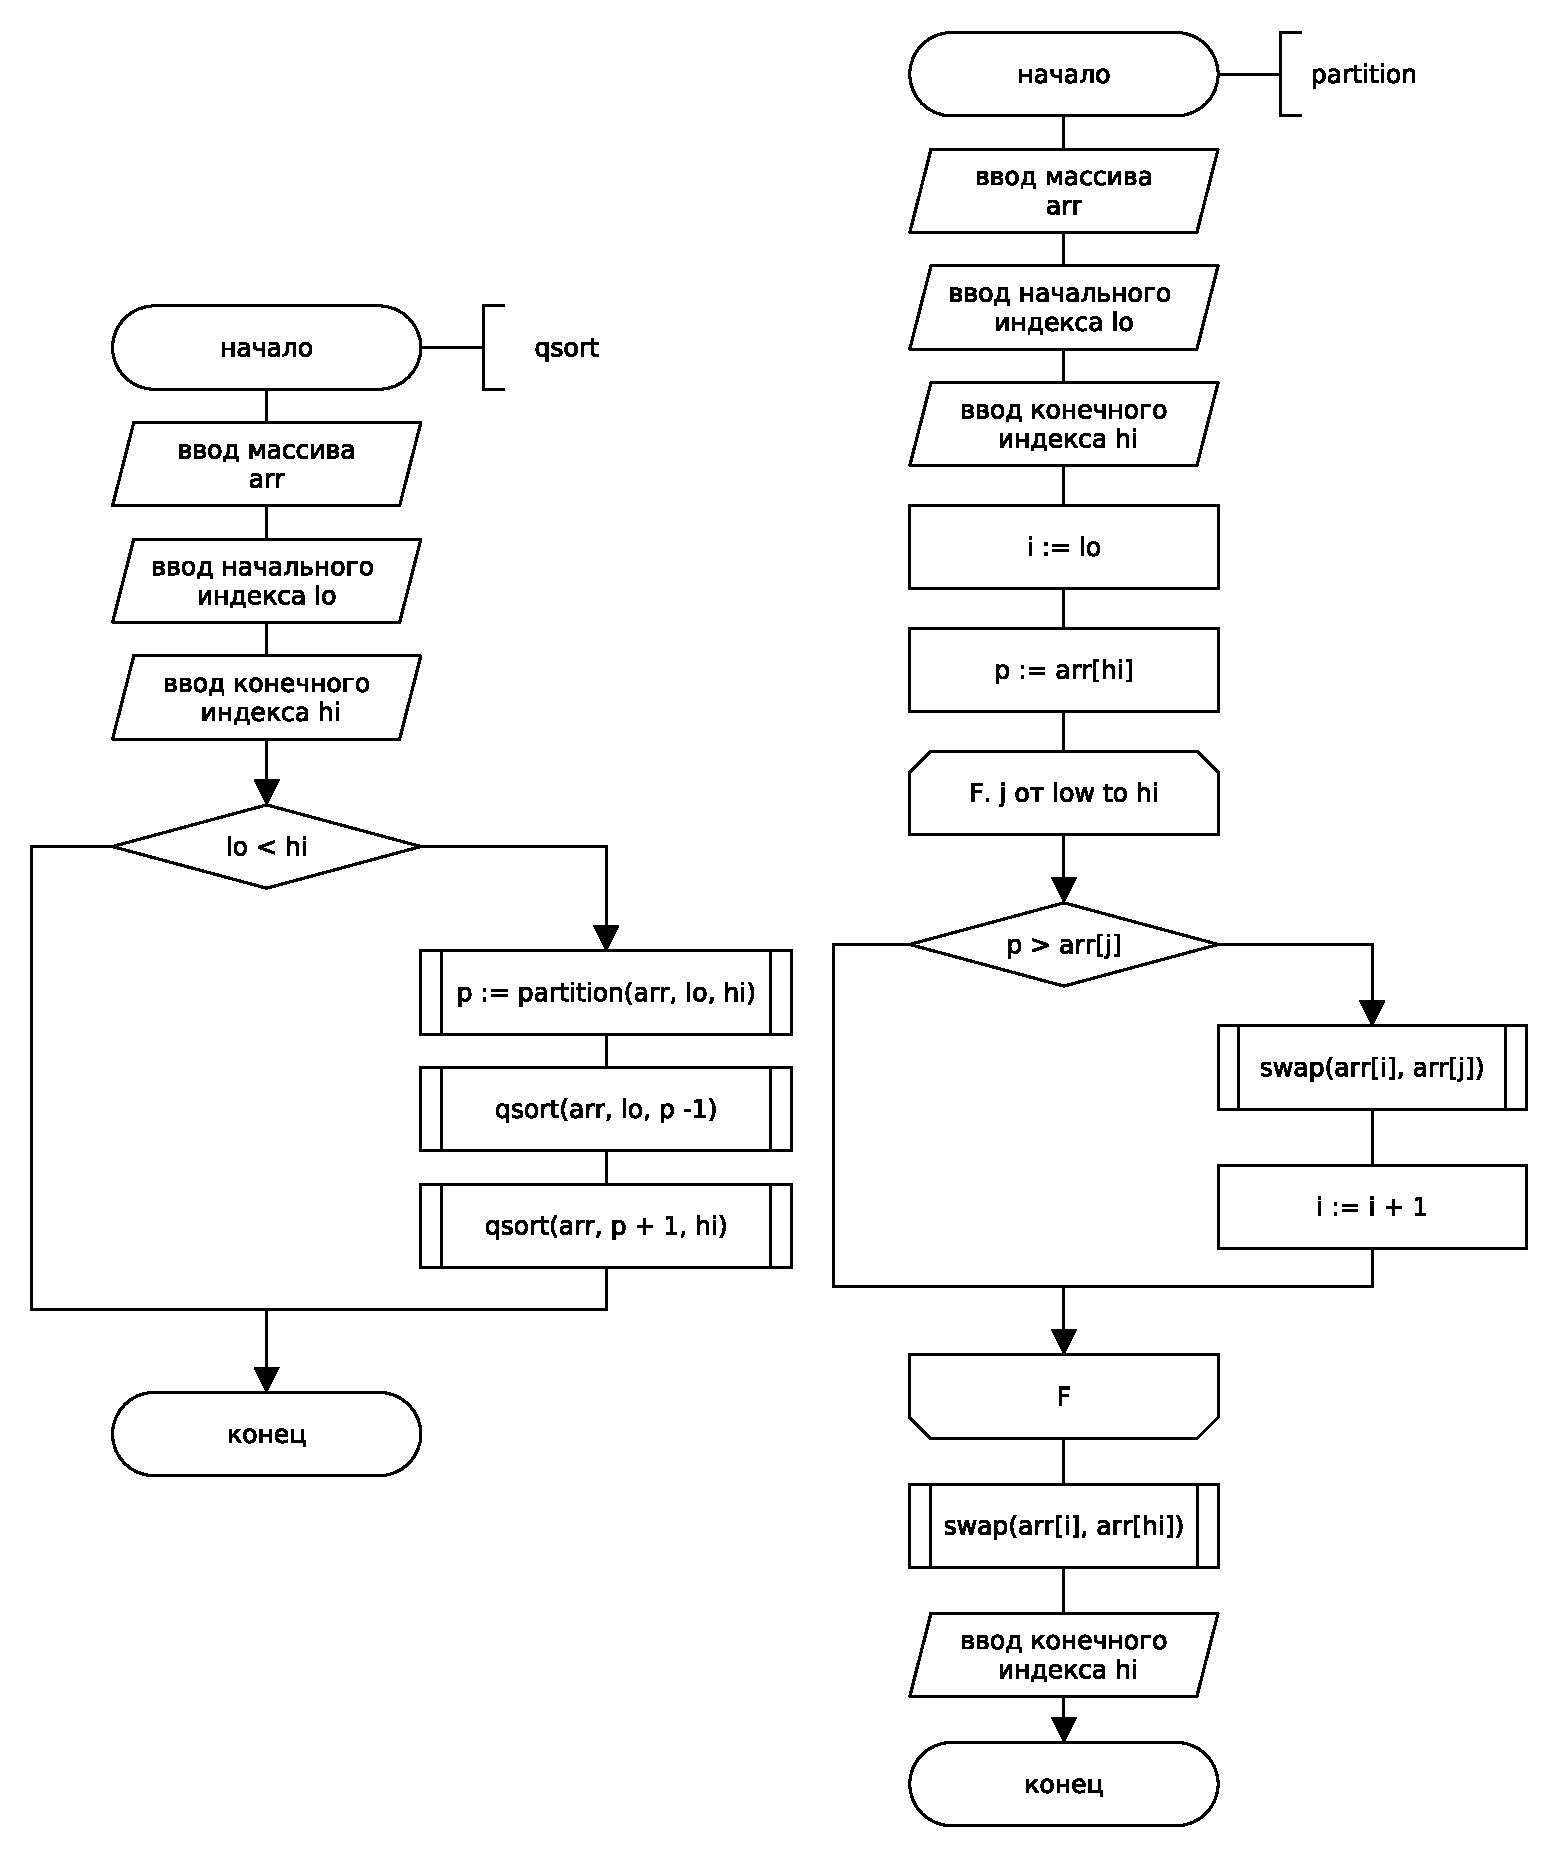
\includegraphics[scale=0.65]{./pdf/qsort.pdf}
    \caption{Быстрая сортровка}
    \label{img:qs}
\end{figure}

\begin{figure}[H]
    \centering
    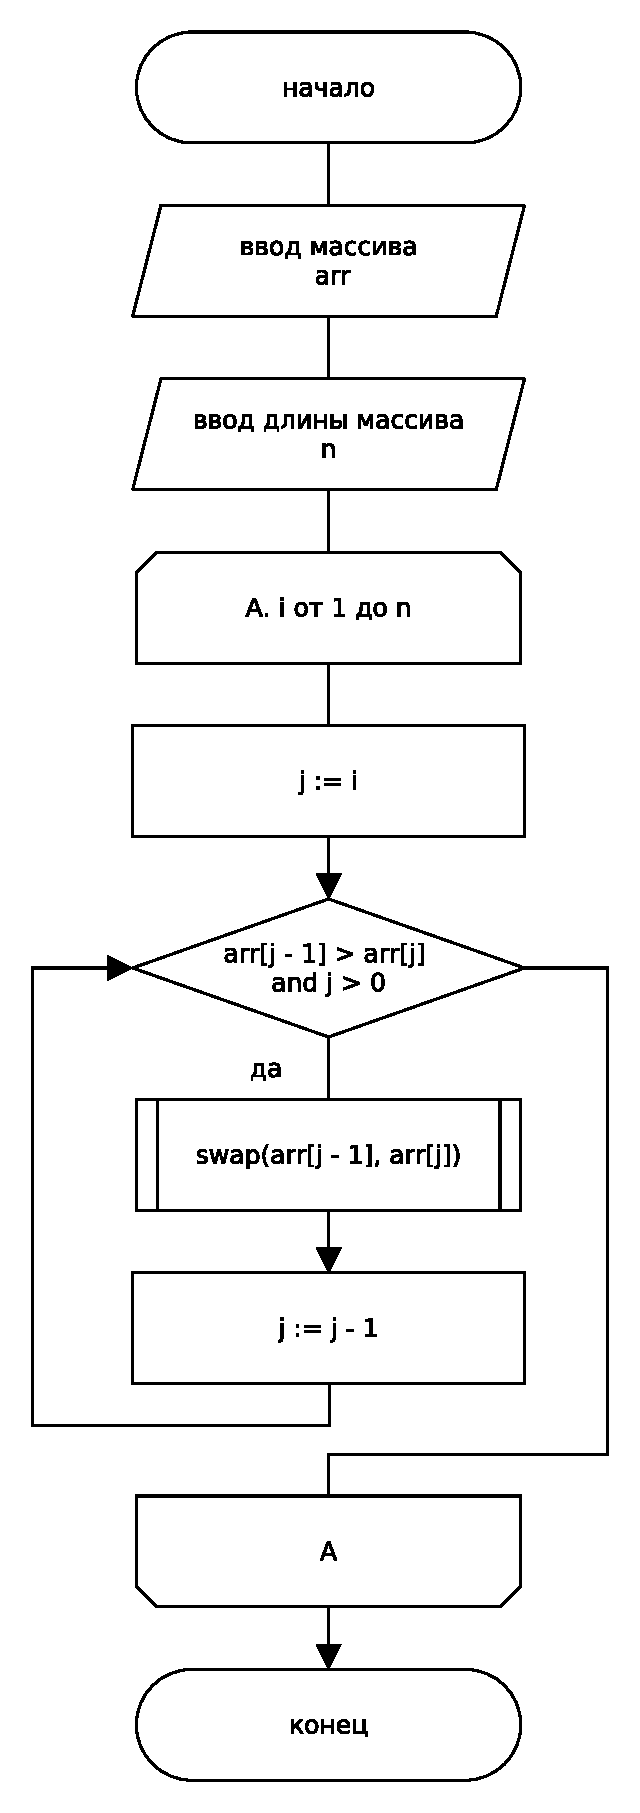
\includegraphics[scale=0.65]{./pdf/insertionsort.pdf}
    \caption{Сортировка вставками}
    \label{img:ins}
\end{figure}

\begin{figure}[H]
    \centering
    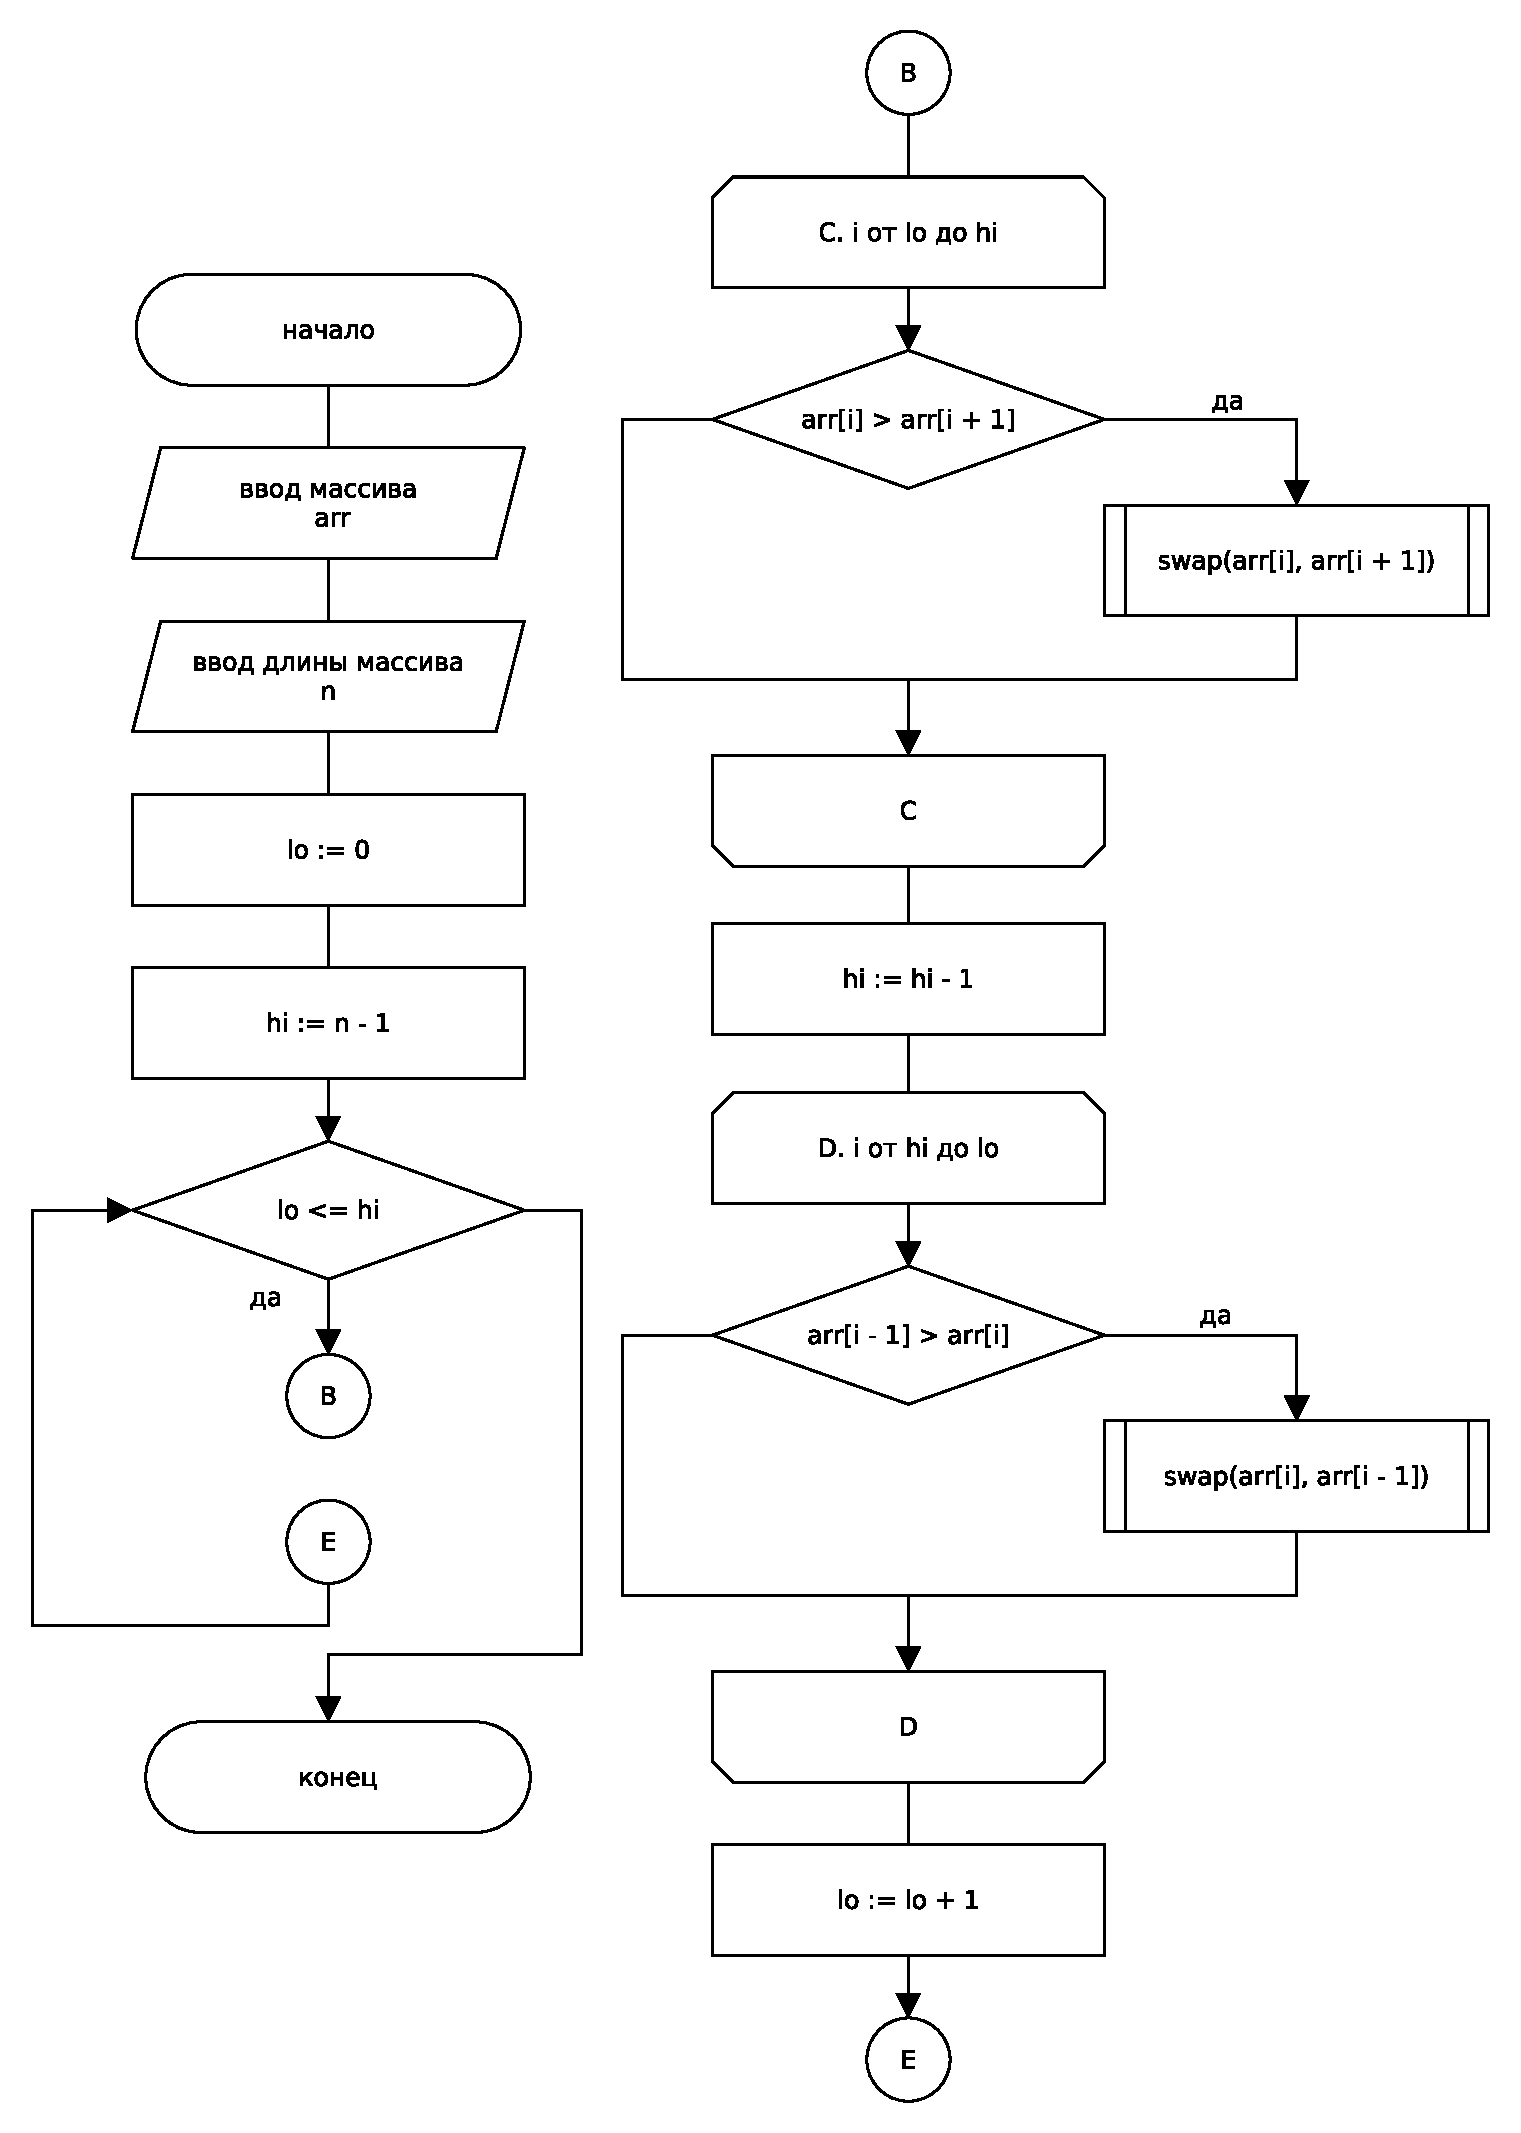
\includegraphics[scale=0.65]{./pdf/shakersort.pdf}
    \caption{Шейкерная сортировка}
    \label{img:shs}
\end{figure}

\section{Трудоемкость алгоритмов}
Проведём оценку сложности рассматриваемых алгоритмов сортировки.

\subsection{Быстрая сортировка}
Быстрая сортировка является рекурсивным алгоритмом, значит при подсчёте стоимости производимых операций будет получено рекуррентное отношение. Для упрощения задачи, подсчитаем асимптотическую сложность лучшего и худшего случаев.

Запишем рекуррентное отношение, соответствующее быстрой сортировке:
\begin{equation}
    T_{qs}(n) = T_{qs}(m) + T_{qs}(s) + f_{partition}(n)
\end{equation}
где $n$ - размер входного массива, $m$ - размер левого подмассива, $s$ - размер правого подмассива, $f_{partition}(n)$ - объём работы, который необходимо совершить, чтобы произвести разбиение массива длины $n$.

Так как мы вычисляем асимптотическую сложность всего алгоритма, то вычислять точную трудоёмкость функции разбиения, его составляющей, не имеет смысла. Разбиение Ломуто заключается в единственном линейном обходе входного массива, а выбор опорного элемента имеет постоянную сложность, потому что это всегда последний элемент. Таким образом имеем сложность функции разбиения $O(n)$, другими словами:
\begin{equation}
    f_{partition}(n) = n
\end{equation}

Лучшим случаем для быстрой сортировки будет тот, при котором глубина дерева рекурсивных вызовов будет минимальна. Это условие будет достигнуто, если на каждом этапе рекурсии входной массив будет разбиваться на два равных (или практически равных) по длине подмассива. Тогда имеем следующие рекуррентное отношение:
\begin{equation}
    T_{qs}(n) = T_{qs}(\frac{n}{2}) + T_{qs}(\frac{n}{2}) + n = 2 \cdot{} T_{qs}(\frac{n}{2}) + n
\end{equation}
Что напоминает вид основной теоремы о рекуррентных соотношениях:
\begin{equation}
    T(n) = a \cdot{} T(\frac{n}{b}) + f(n)
\end{equation}
где $a = 2$, $b = 2$, $f(n) = n$. Это означает, что применив эту теорему мы получим искомую трудоёмкость. Очевидно, первый варианты основной теоремы рекуррентных соотношений не подходит, так как:
\begin{equation}
    f(n) = n = n^1 = n^c \Rightarrow{} c = 1 = log_2(2) = log_b(a) \Rightarrow c \nless{} log_b(a)
\end{equation}

Проверим второй вариант:
\begin{equation}
    f(n) = n = n^1 = n^1 \cdot{} log^0(n) = n^c \cdot{} log^k(n)
\end{equation}
где $c = 1 = log_b(a)$, $k = 0$, а значит условия второго варианта основной теоремы соблюдены. Таким образом имеем асимптотическую сложность быстрой сортировки с разбиением Ломуто в лучшем случае:
\begin{equation}
    T_{qs} = O(n \cdot{} log(n))
\end{equation}

Рассмотрим худший случай. Условия его наступления полностью противоположны условиям лучшего случая: глубина дерева рекурсивных вызовов должна быть максимальна. Это означает, что в ходе первого разбиения будут получены подмассивы длин $1$ и $n - 1$, а на всех последующих этапах рекурсии длина большего подмассива будет уменьшаться только на 1, а общее число операций разбиения составит $n - 1$. Тогда можем подсчитать трудоёмкость:
\begin{equation}
    \sum_{i = 0}^{n - 1}(n - i) \approx O(n^2)
\end{equation}

Таким образом сортировка полностью отсортированного массива или обратно отсортированного массива является худшим случаем для быстрой сортировки с выбором последнего элемента в качестве опорного, а её сложность равна $O(n^2)$.

Сложность выполнения быстрой сортировки в среднем случае имеет вероятностный характер, так как в произвольном массиве отношение порядка, в котором находятся соседние элементы, случайно. Имеем трудоёмкость\cite{knuth}:
\begin{equation}
    O(n \cdot{} log(n))
\end{equation}

\subsection{Сортировка вставками}
Изображённый на рисунке \ref{img:ins} алгоритм сортировки вставками состоит из двух вложенных циклов. В лучшем случае внутренний цикл вырождается, а в худшем - всегда выполняется. Этим событиям соответствуют обработка отсортированного массива и обратно отсортированного.

Трудоёмкость лучшего случая:
\begin{equation}
    2 + (n - 1) \cdot{} (4 + 5) = 2 + (n - 1) \cdot{} 9 = 9n - 7
\end{equation}
Тут $n$ - это длина сортируемого массива.

Трудоёмкость худшего случая:
\begin{equation}
    2 + (n - 1) \cdot{} (4 + (n - 1) \cdot{} (9 + 3)) = 11n^2 - 18n + 9
\end{equation}

Значит, асимптотическая сложность для лучшего случая - $O(n)$, для худшего - $O(n^2)$, а для среднего - $O(n^2)$\cite{knuth}.

\subsection{Шейкерная сортировка}
Шейкерная сортировка в любых случаях имеет асимптотическую сложность $O(n^2)$\cite{knuth}. Причина этого заключается в том, что количество итераций вложенных циклов данного алгоритма зависит только от количества входных данных, но не от степени их упорядоченности. Но существует модификация, которая сделает асимптотическую сложность алгоритма шейкерной сортировки идентичной таковой для сортировки вставками: после выполнения вложенных циклов, если не произошло ни одного обмена, завершить сортировку.

\section{Вывод}
Быстрая сортировка имеет лучшую среднюю сложность, что говорит о ней, как о потенциально наиболее универсальной сортировке. Шейкреная сортировка имеет наихудшую трудоёмкость во всех случаях, а значит его применение нецелесообразно в принципе.

